\documentclass[a4paper, 12pt]{article}
\usepackage[UTF8]{ctex}
\usepackage{geometry}
\usepackage{graphicx}
\usepackage{float}
\usepackage{hyperref}
\usepackage{tcolorbox}
\tcbuselibrary{most}

% 设置页边距
\geometry{a4paper, left=2.5cm, right=2.5cm, top=2.5cm, bottom=2.5cm}

% 简化实例方框样式
\tcbset{instancestyle/.style={
    enhanced,
    sharp corners,
    colback=white,
    colframe=black!70!white,
    boxrule=0.8pt,
    left=6pt,
    right=6pt,
    top=6pt,
    bottom=6pt,
    boxsep=2pt,
    arc=2pt
}}

\begin{document}

\title{\huge{系统开发工具基础实验报告3}}
\author{姓名:\underline{刘浩洋} \\ 
        学号:\underline{24040021022} \\ 
        班级:\underline{软件工程}}
\date{实验日期:\underline{2025年9月12日}}
\maketitle

\section*{一、实验目的}
\begin{enumerate}
    \item 掌握Linux命令行中任务与进程的管理方法,包括前台/后台切换、暂停、恢复与终止;
    \item 熟悉Python基本语法,掌握变量、控制结构、函数和模块的使用;
    \item 初步了解OpenCV库的基本功能,实现图像的读取、显示与简单处理;
\end{enumerate}

\section*{二、实验环境}
\begin{itemize}
    \item 操作系统:Windows 11
    \item 虚拟化平台:VMware Workstation Pro 17
    \item 虚拟机系统:Ubuntu 24.04.3 LTS(64位)
    \item Shell环境:Bash
    \item 编程语言:Python 3
    \item 图像处理库:OpenCV-Python (cv2)
\end{itemize}

\section*{三、练习内容}
本次实验主要包括:
\begin{itemize}
    \item 使用Shell进行进程的启动、暂停、后台运行与信号控制;
    \item 编写Python脚本实现基本逻辑与函数调用;
    \item 使用OpenCV进行图像的加载、显示与颜色空间转换;
    \item 结合count.py和fib.py演示任务控制机制;
\end{itemize}

\section*{四、20个实例(命令行、Python与OpenCV)}

\begin{tcolorbox}[instancestyle, title=实例1:创建实验目录结构]
为组织本次实验文件,创建包含子目录的项目结构。
使用 -p 参数可安全创建多级目录。

\texttt{mkdir -p /home/lhy/lesson3/\{scripts,images,docs\}} \\
\texttt{cd /home/lhy/lesson3} \\
\texttt{touch scripts/count.py scripts/fib.py} \\
\texttt{ls -R} \\
\texttt{pwd}
\end{tcolorbox}

\begin{tcolorbox}[instancestyle, title=实例2:编写count.py(无限计数)]
编写一个持续输出递增数字的Python脚本,
用于演示长时间运行任务的进程控制。

\texttt{\#!/usr/bin/env python3} \\
\texttt{import time} \\
\texttt{print("开始计数")} \\
\texttt{number = 1} \\
\texttt{while True:} \\
\texttt{    print(number)} \\
\texttt{    number += 1} \\
\texttt{    time.sleep(2)}
\end{tcolorbox}

\begin{tcolorbox}[instancestyle, title=实例3:编写fib.py(斐波那契计算)]
编写一个计算前50项斐波那契数列的脚本,
用于演示耗时任务的后台运行与监控。

\texttt{\#!/usr/bin/env python3} \\
\texttt{import time} \\
\texttt{def fb(n):} \\
\texttt{    if n == 1 or n == 2:} \\
\texttt{        return 1} \\
\texttt{    return fb(n-1) + fb(n-2)} \\
\texttt{start = time.time()} \\
\texttt{for i in range(1, 51):} \\
\texttt{    time.sleep(2)} \\
\texttt{    print('fb(\%d)=\%d' \% (i, fb(i)))} \\
\texttt{end = time.time()} \\
\texttt{print('总时间为: \%fs' \% (end - start))}
\end{tcolorbox}

\begin{tcolorbox}[instancestyle, title=实例4:在前台运行Python脚本]
直接执行脚本,它将在前台占用终端,
期间无法输入其他命令,按 Ctrl+C 可中断。

\texttt{python3 scripts/count.py}
\end{tcolorbox}

\begin{tcolorbox}[instancestyle, title=实例5:暂停前台任务(Ctrl+Z)]
在脚本运行时按 \texttt{Ctrl+Z},
可将任务暂停并送入后台,状态为 Stopped。

\texttt{\# 运行中按 Ctrl+Z} \\
\texttt{[1]+  Stopped                 python3 scripts/count.py}
\end{tcolorbox}

\begin{tcolorbox}[instancestyle, title=实例6:后台运行脚本(\&)]
在命令末尾加 \&,可让脚本在后台运行,
终端立即返回,可继续执行其他命令。

\texttt{python3 scripts/fib.py \&} \\
\texttt{[1] 12345} \\
\texttt{\# 脚本在后台运行,PID为12345}
\end{tcolorbox}

\begin{tcolorbox}[instancestyle, title=实例7:查看后台任务(jobs)]
使用 jobs 命令查看当前Shell会话中的后台任务,
包括运行中和暂停的任务及其状态。

\texttt{jobs} \\
\texttt{[1]+  Running    python3 scripts/fib.py \&} \\
\texttt{[2]-  Stopped    python3 scripts/count.py}
\end{tcolorbox}

\begin{tcolorbox}[instancestyle, title=实例8:恢复暂停任务到后台(bg)]
使用 bg 命令可将暂停的任务在后台继续运行。

\texttt{bg \%2} \\
\texttt{[2]+ python3 scripts/count.py \&}
\end{tcolorbox}

\begin{tcolorbox}[instancestyle, title=实例9:将后台任务调回前台(fg)]
使用 fg 命令可将后台任务(运行或暂停)调回前台继续交互。

\texttt{fg \%1} \\
\texttt{\# fib.py 恢复到前台,终端被占用}
\end{tcolorbox}

\begin{tcolorbox}[instancestyle, title=实例10:终止进程(kill)]
使用 kill 命令向进程发送信号。
默认发送 SIGTERM,-9 为强制终止 SIGKILL。

\texttt{kill \%1} \\
\texttt{kill -9 12345} \\
\texttt{jobs} \\
\texttt{\# 查看是否已终止}
\end{tcolorbox}

\begin{tcolorbox}[instancestyle, title=实例11:Python变量与数据类型]
Python支持动态类型,常用类型包括int、float、str、bool。

\texttt{\#!/usr/bin/env python3} \\
\texttt{name = "刘浩洋"} \\
\texttt{age = 20} \\
\texttt{height = 1.75} \\
\texttt{isstudent = True} \\
\texttt{print(f"姓名:\{name}, 年龄:\{age}")} \\
\texttt{print(f"身高:\{height}m, 学生:\{isstudent}")}
\end{tcolorbox}

\begin{tcolorbox}[instancestyle, title=实例12:Python控制结构(if-elif-else)]
使用条件语句实现逻辑分支,注意缩进。

\texttt{\#!/usr/bin/env python3} \\
\texttt{score = 85} \\
\texttt{if score >= 90:} \\
\texttt{    print("优秀")} \\
\texttt{elif score >= 80:} \\
\texttt{    print("良好")} \\
\texttt{elif score >= 60:} \\
\texttt{    print("及格")} \\
\texttt{else:} \\
\texttt{    print("不及格")}
\end{tcolorbox}

\begin{tcolorbox}[instancestyle, title=实例13:Python循环(for与while)]
for 循环常用于遍历序列,while 用于条件循环。

\texttt{\#!/usr/bin/env python3} \\
\texttt{# for循环} \\
\texttt{fruits = ["苹果", "香蕉", "橙子"]} \\
\texttt{for fruit in fruits:} \\
\texttt{    print(f"我喜欢\{fruit}")} \\
\texttt{} \\
\texttt{\# while循环} \\
\texttt{i = 0} \\
\texttt{while i < 3:} \\
\texttt{    print(f"计数:\{i}")} \\
\texttt{    i += 1}
\end{tcolorbox}

\begin{tcolorbox}[instancestyle, title=实例14:Python函数定义与调用]
函数用于封装可复用代码,支持参数与返回值。

\texttt{\#!/usr/bin/env python3} \\
\texttt{def greet(name, lang="中文"):\\
\texttt{    return f"你好,\{name}!使用\{lang}打招呼。"} \\
\texttt{} \\
\texttt{print(greet("张三"))} \\
\texttt{print(greet("李四", "Python"))}
\end{tcolorbox}

\begin{tcolorbox}[instancestyle, title=实例15:导入Python模块]
使用 import 导入标准库或第三方库。

\texttt{\#!/usr/bin/env python3} \\
\texttt{import math} \\
\texttt{import datetime} \\
\texttt{} \\
\texttt{print("圆周率:", math.pi)} \\
\texttt{print("当前时间:", datetime.datetime.now())}
\end{tcolorbox}

\begin{tcolorbox}[instancestyle, title=实例16:安装OpenCV库]
使用 pip 安装 OpenCV-Python 库,
需确保已安装 pip 和相关依赖。

\texttt{sudo apt update} \\
\texttt{sudo apt install python3-pip} \\
\texttt{pip3 install opencv-python}
\end{tcolorbox}

\begin{tcolorbox}[instancestyle, title=实例17:读取并显示图像(OpenCV)]
使用cv2.imread()读取图像,cv2.imshow()显示。

\texttt{\#!/usr/bin/env python3} \\
\texttt{import cv2} \\
\texttt{img = cv2.imread("images/test.jpg")} \\
\texttt{if img is not None:} \\
\texttt{    cv2.imshow("图像", img)} \\
\texttt{    cv2.waitKey(0)} \\
\texttt{    cv2.destroyAllWindows()} \\
\texttt{else:} \\
\texttt{    print("图像加载失败!")}
\end{tcolorbox}

\begin{tcolorbox}[instancestyle, title=实例18:图像亮度调整]
使用 cv2.convertScaleAbs() 调整图像亮度。
通过 input 获取用户输入的亮度值(-100 到 100),
负值变暗,正值变亮,处理后保存为 pic.png。

\texttt{\#!/usr/bin/env python3} \\
\texttt{import cv2} \\
\texttt{img = cv2.imread("images/test.jpg")} \\
\texttt{if img is None:} \\
\texttt{    print("错误:图像加载失败,请检查路径!")} \\
\texttt{else:} \\
\texttt{    value = int(input("亮度值(-100到100): "))} \\
\texttt{    img\_adjusted = cv2.convertScaleAbs(img, beta=value)} \\
\texttt{    cv2.imwrite("pic.png", img\_adjusted)} \\
\texttt{    print("亮度已调整并保存")}
\end{tcolorbox}

\begin{tcolorbox}[instancestyle, title=实例19:保存处理后的图像]
使用cv2.imwrite()将处理结果保存到文件。

\texttt{\#!/usr/bin/env python3} \\
\texttt{import cv2} \\
\texttt{img = cv2.imread("images/test.jpg")} \\
\texttt{gray = cv2.cvtColor(img, cv2.COLOR_BGR2GRAY)} \\
\texttt{cv2.imwrite("images/gray.jpg", gray)} \\
\texttt{print("灰度图像已保存!")}
\end{tcolorbox}

\begin{tcolorbox}[instancestyle, title=实例20:综合任务控制演示]
综合使用count.py和fib.py演示完整任务控制流程。

\texttt{\# 1. 后台运行计数} \\
\texttt{python3 scripts/count.py \&} \\
\texttt{\# 2. 后台运行斐波那契} \\
\texttt{python3 scripts/fib.py \&} \\
\texttt{\# 3. 查看任务} \\
\texttt{jobs} \\
\texttt{\# 4. 暂停其中一个} \\
\texttt{kill -STOP \%1} \\
\texttt{\# 5. 恢复} \\
\texttt{kill -CONT \%1} \\
\texttt{\# 6. 终止全部} \\
\texttt{kill \%1 \%2}
\end{tcolorbox}

\newpage

\begin{figure}[htbp]
    \centering
    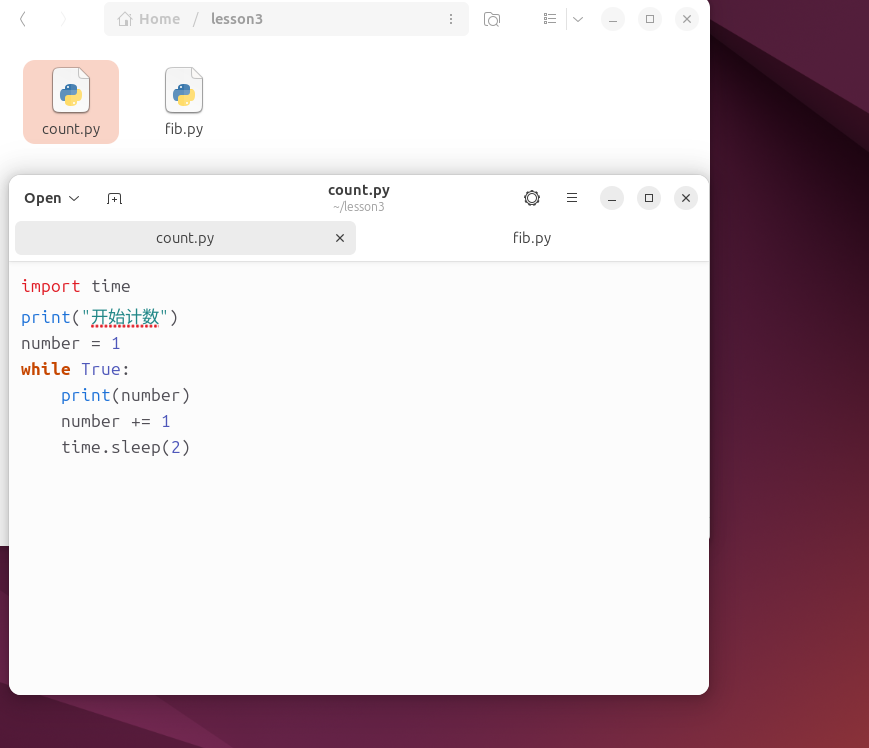
\includegraphics[width=0.8\textwidth]{lec3 (1).png}
    \caption{lec3-1}
    \label{fig:lec3-1}
\end{figure}

\begin{figure}[htbp]
    \centering
    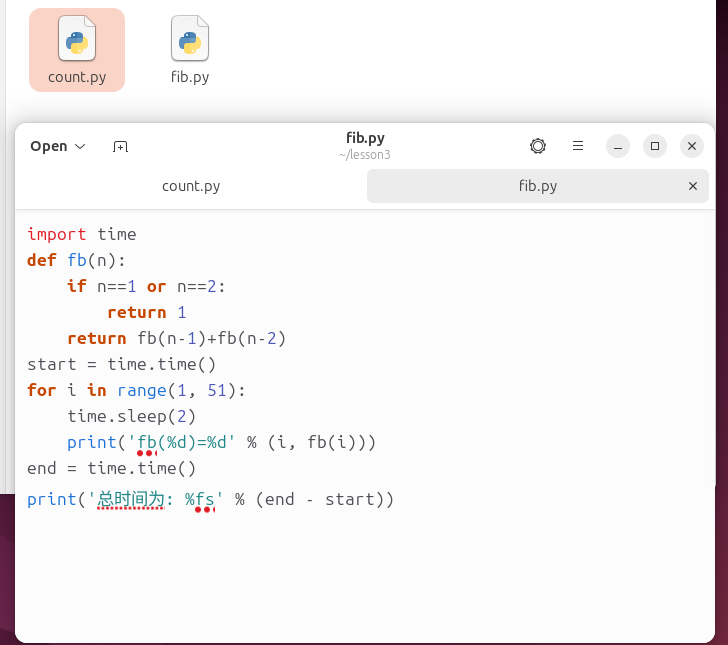
\includegraphics[width=0.8\textwidth]{lec3 (2).png}}
    \caption{lec3-2}
    \label{fig:lec3-2}
\end{figure}

\begin{figure}[htbp]
    \centering
    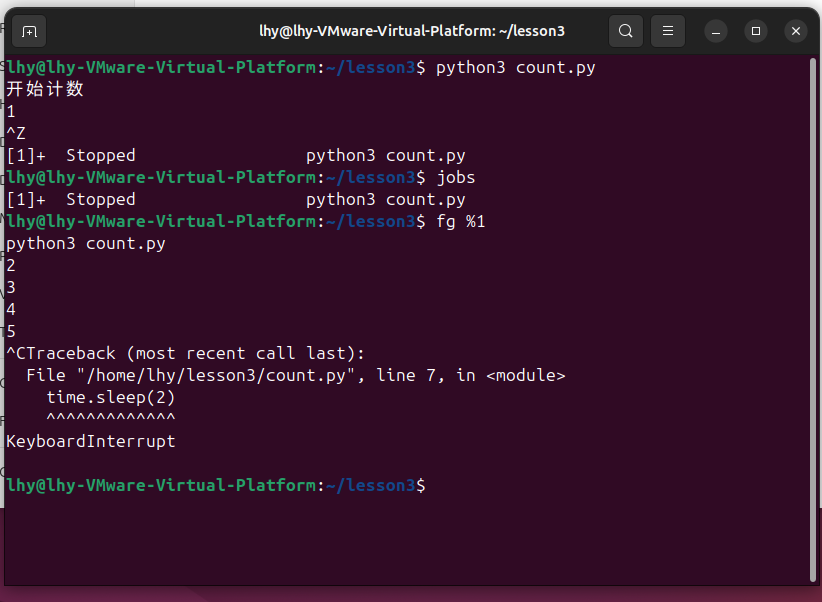
\includegraphics[width=0.8\textwidth]{lec3 (3).png}}
    \caption{lec3-3}
    \label{fig:lec3-3}
\end{figure}

\begin{figure}[htbp]
    \centering
    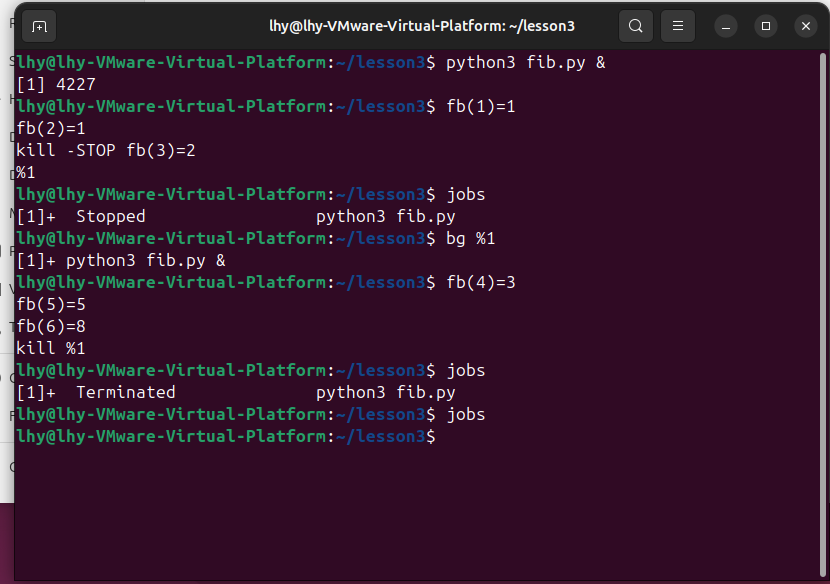
\includegraphics[width=0.8\textwidth]{lec3 (4).png}}
    \caption{lec3-4}
    \label{fig:lec3-4}
\end{figure}

\begin{figure}[htbp]
    \centering
    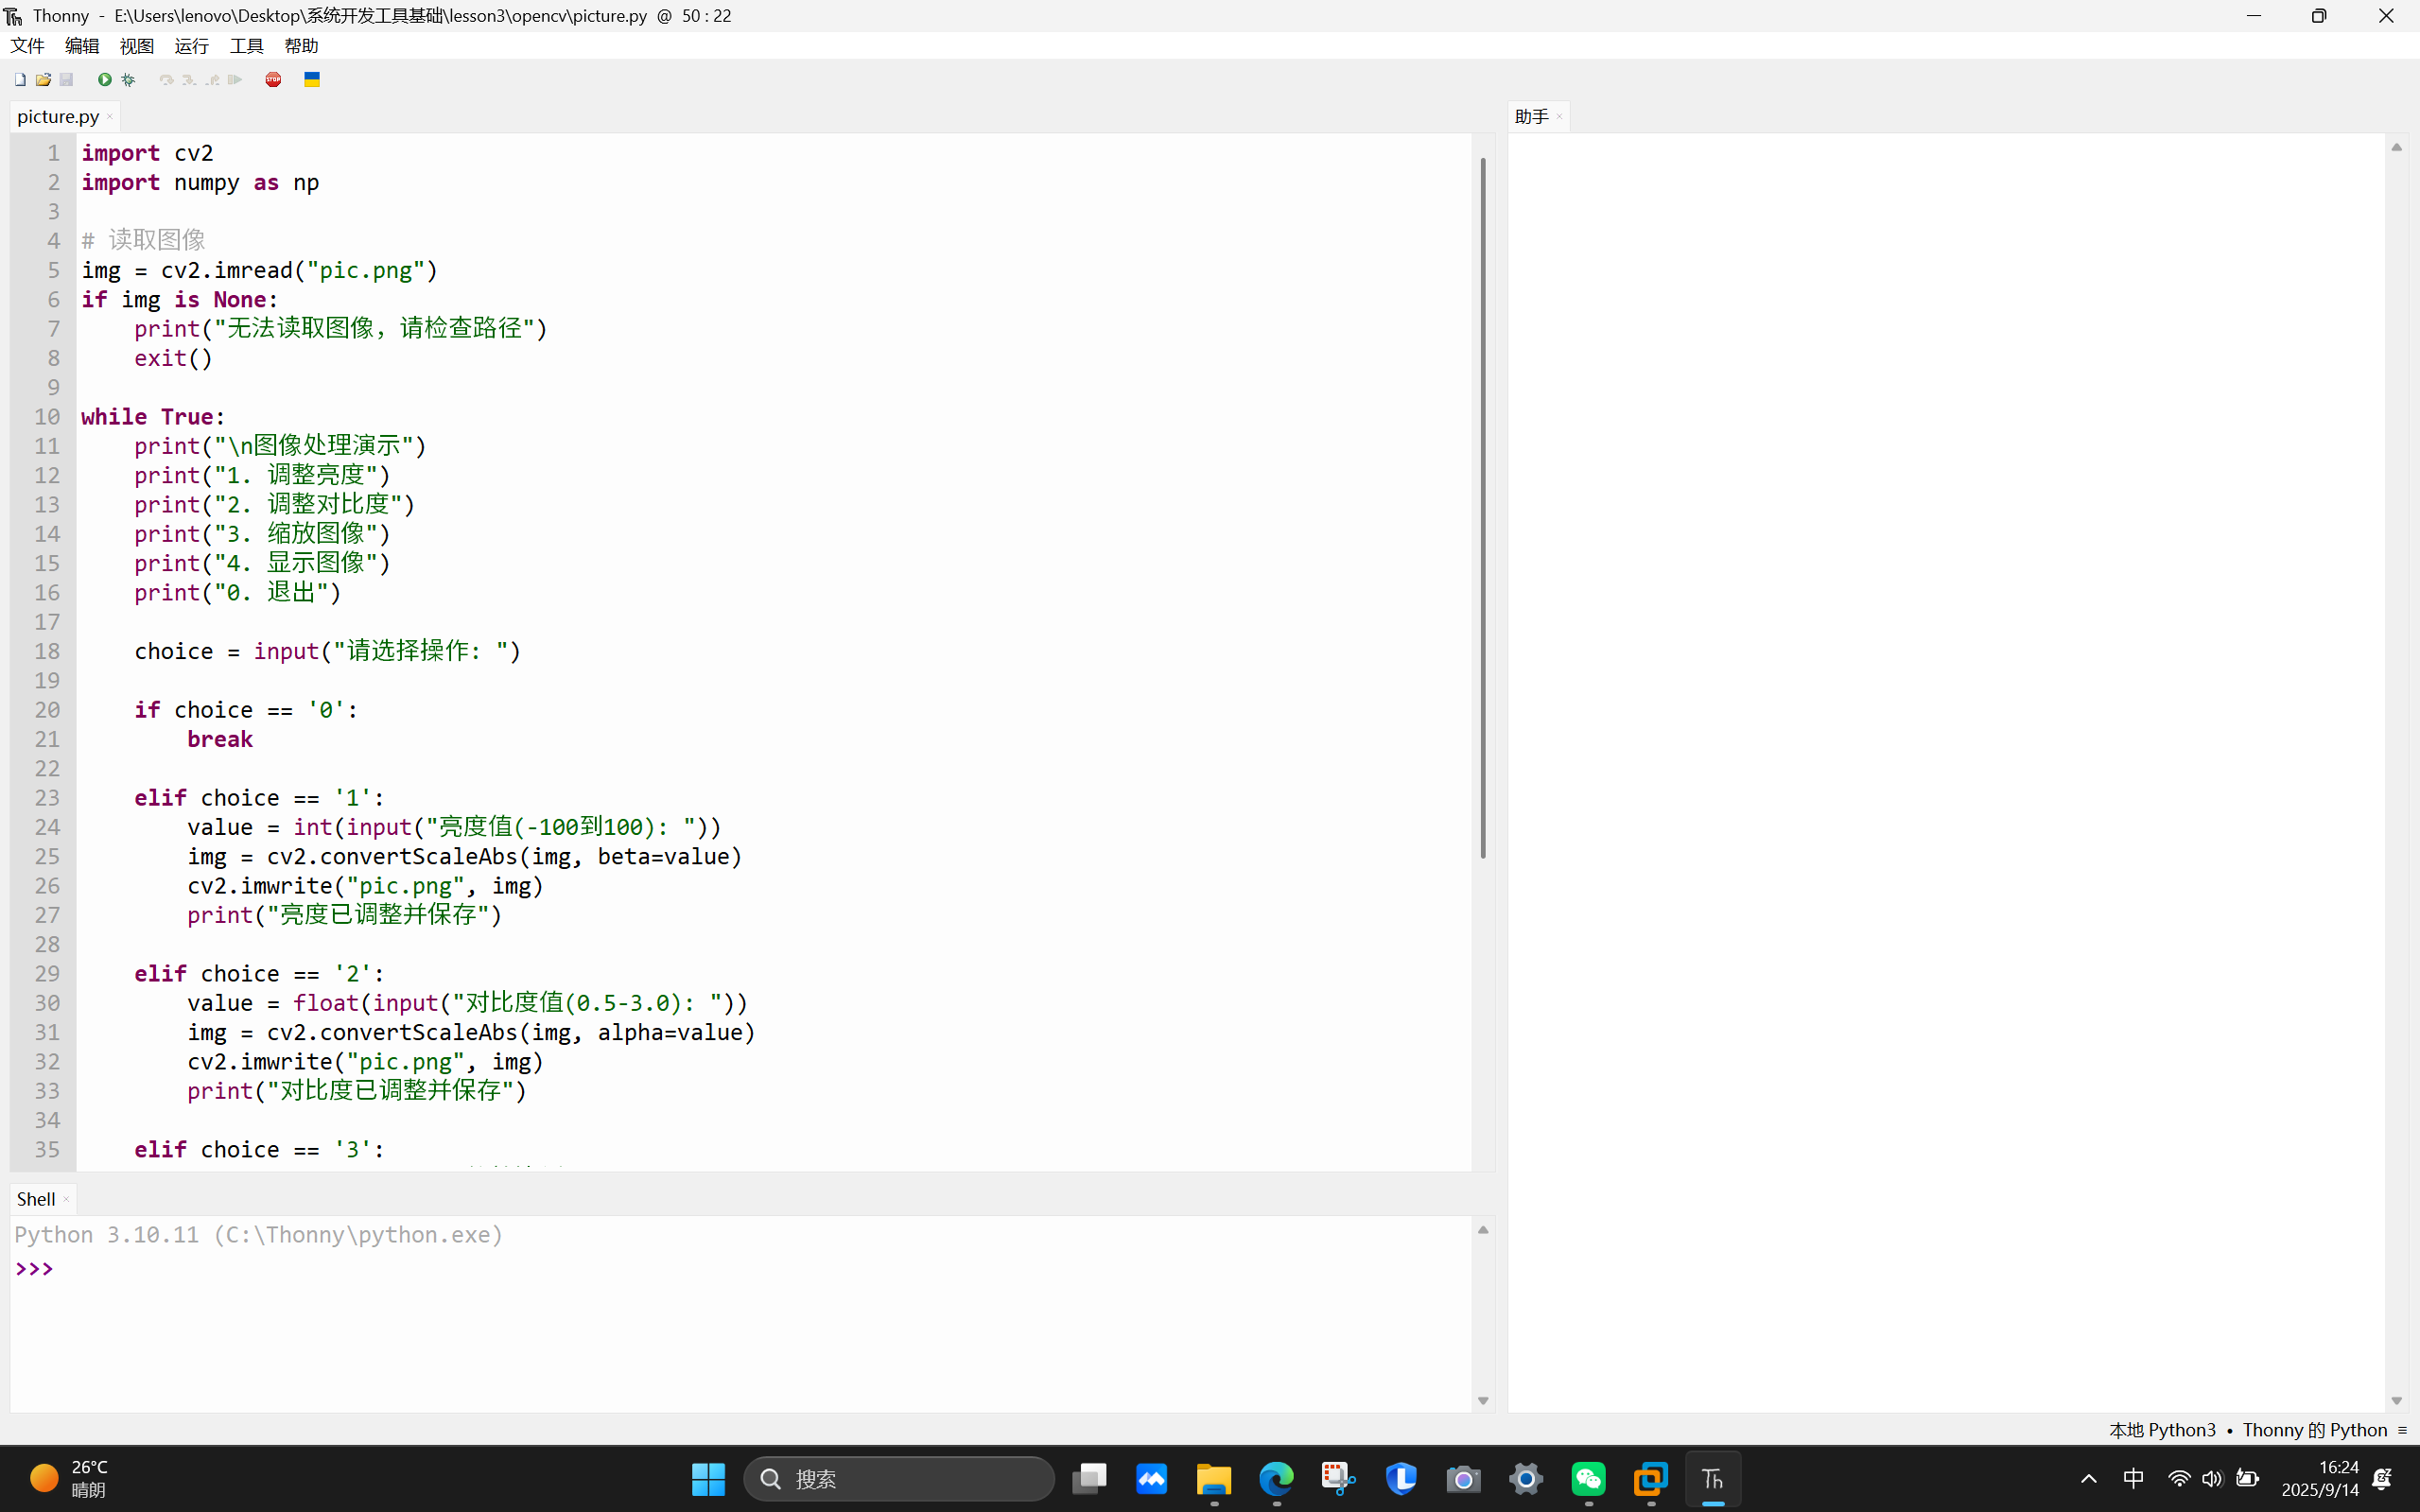
\includegraphics[width=0.8\textwidth]{lec3 (5).png}}
    \caption{lec3-5}
    \label{fig:lec3-5}
\end{figure}

\begin{figure}[htbp]
    \centering
    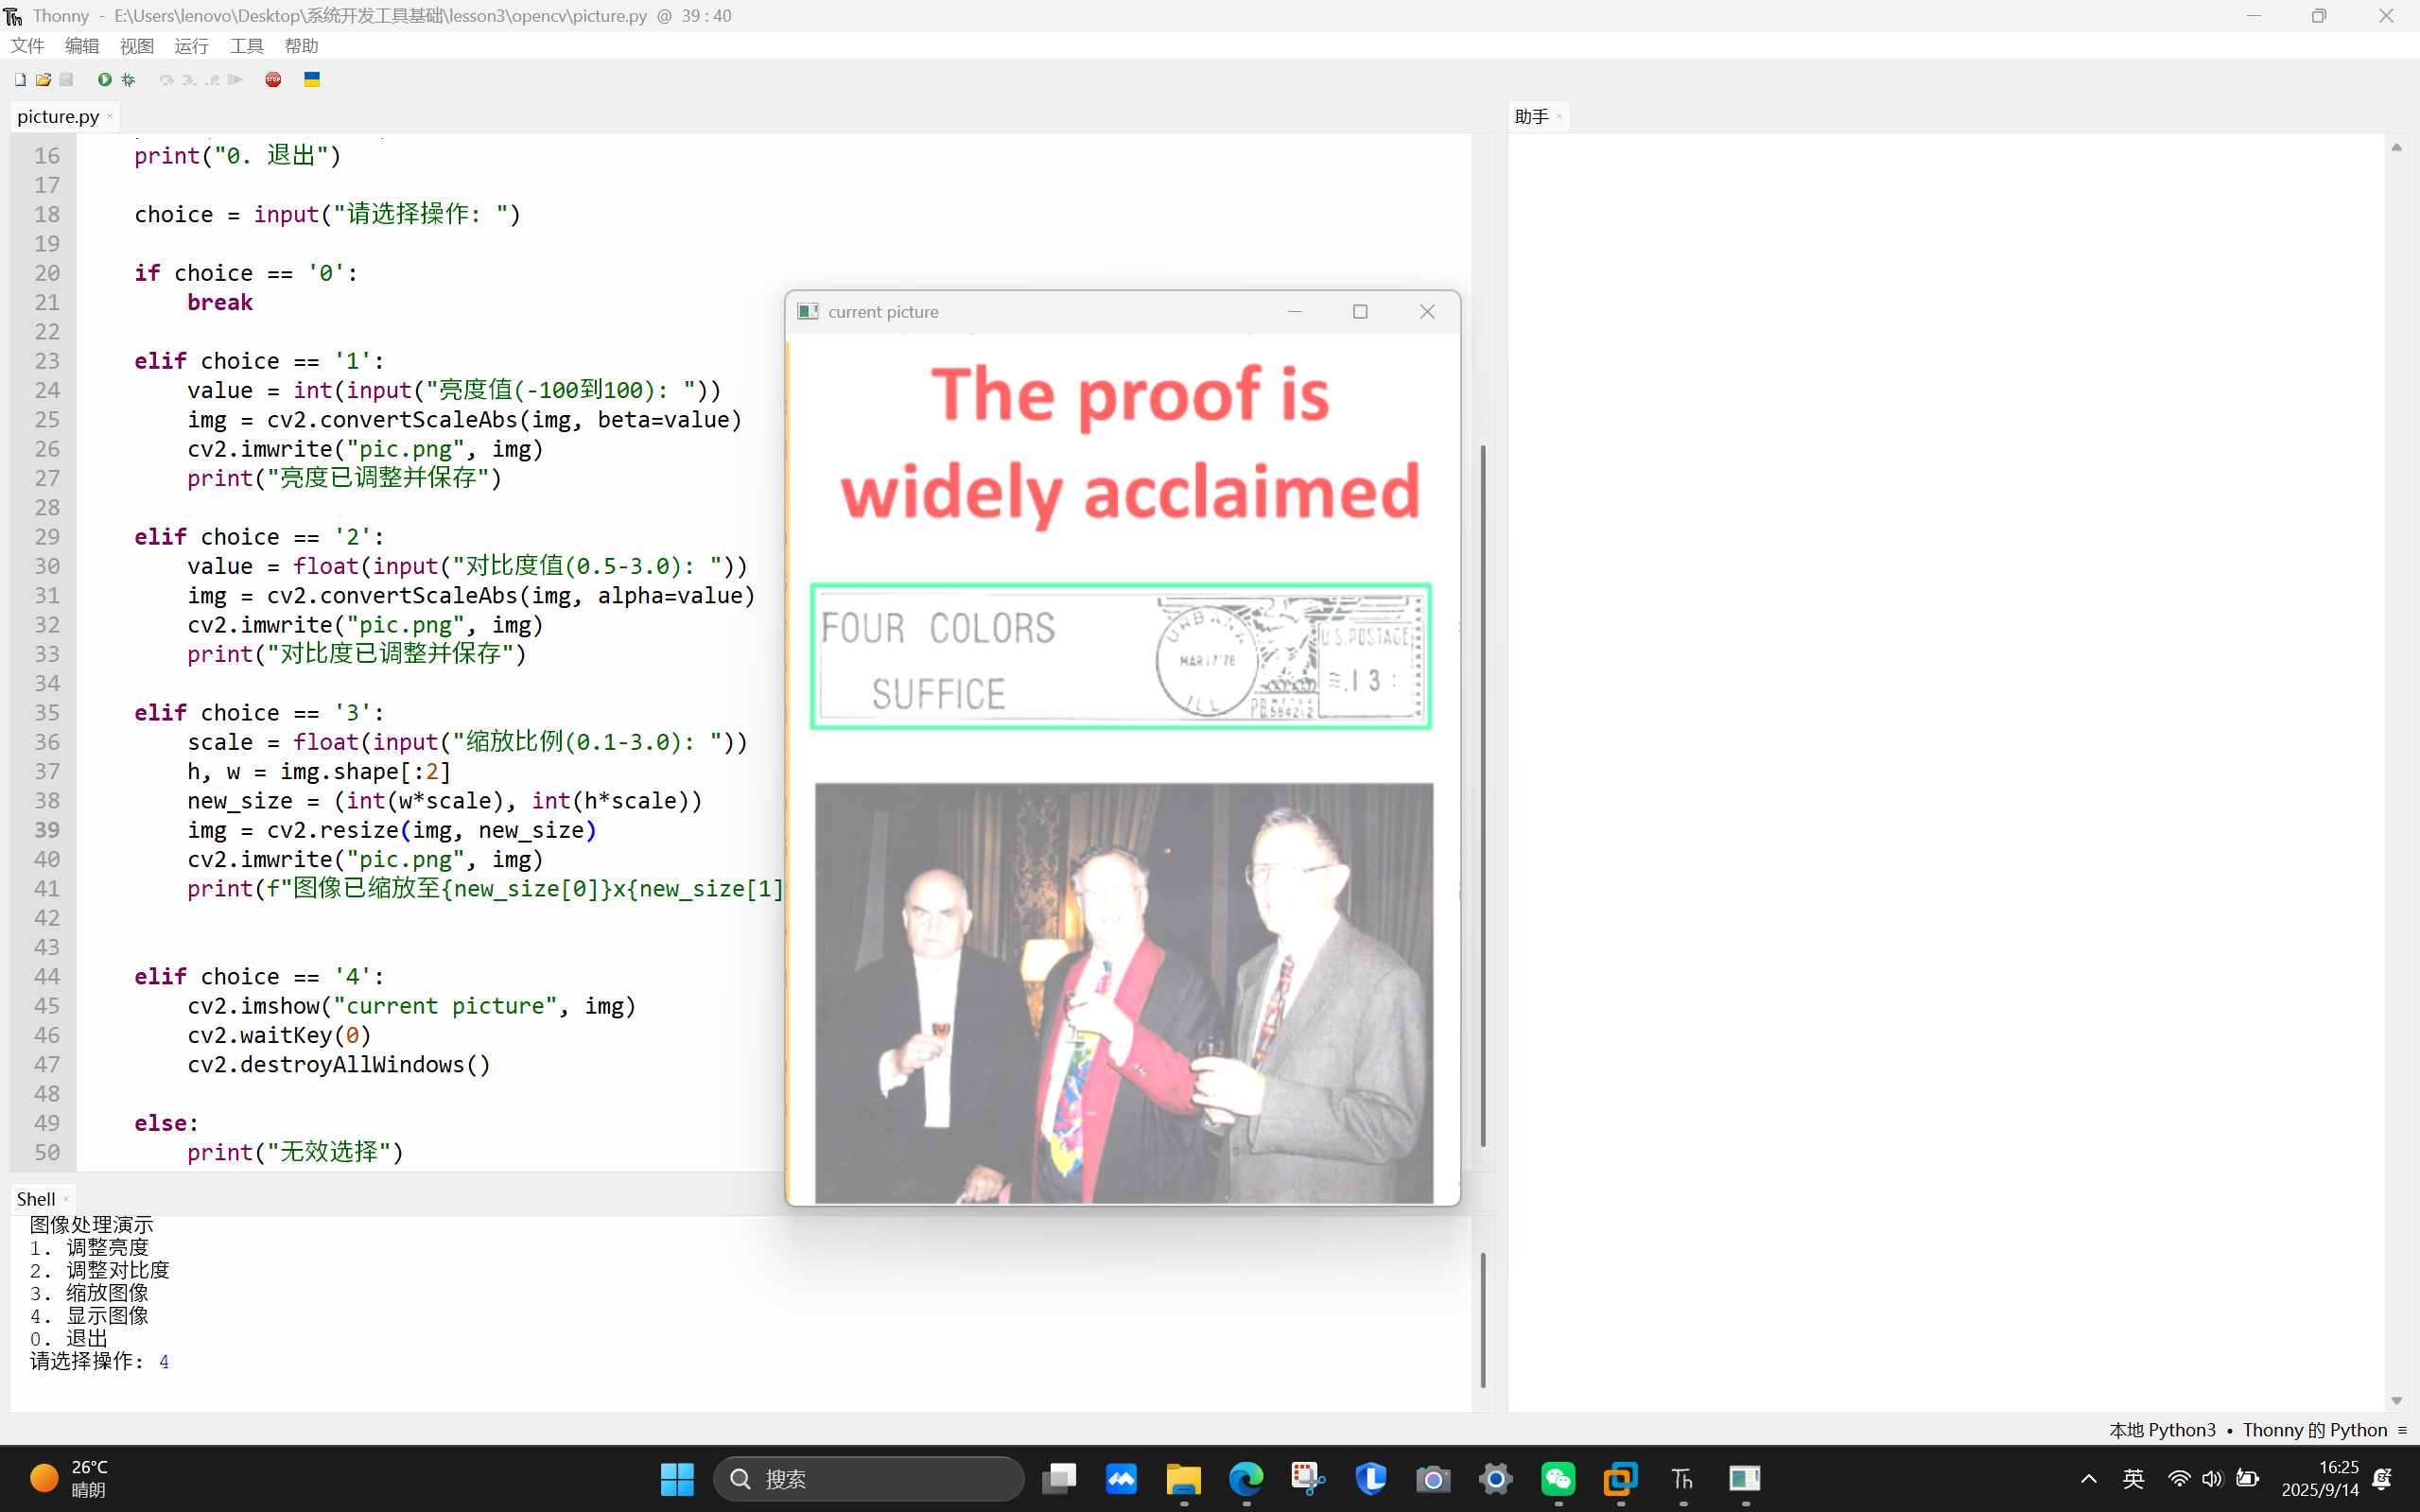
\includegraphics[width=0.8\textwidth]{lec3 (6).png}}
    \caption{lec3-6}
    \label{fig:lec3-6}
\end{figure}

\begin{figure}[htbp]
    \centering
    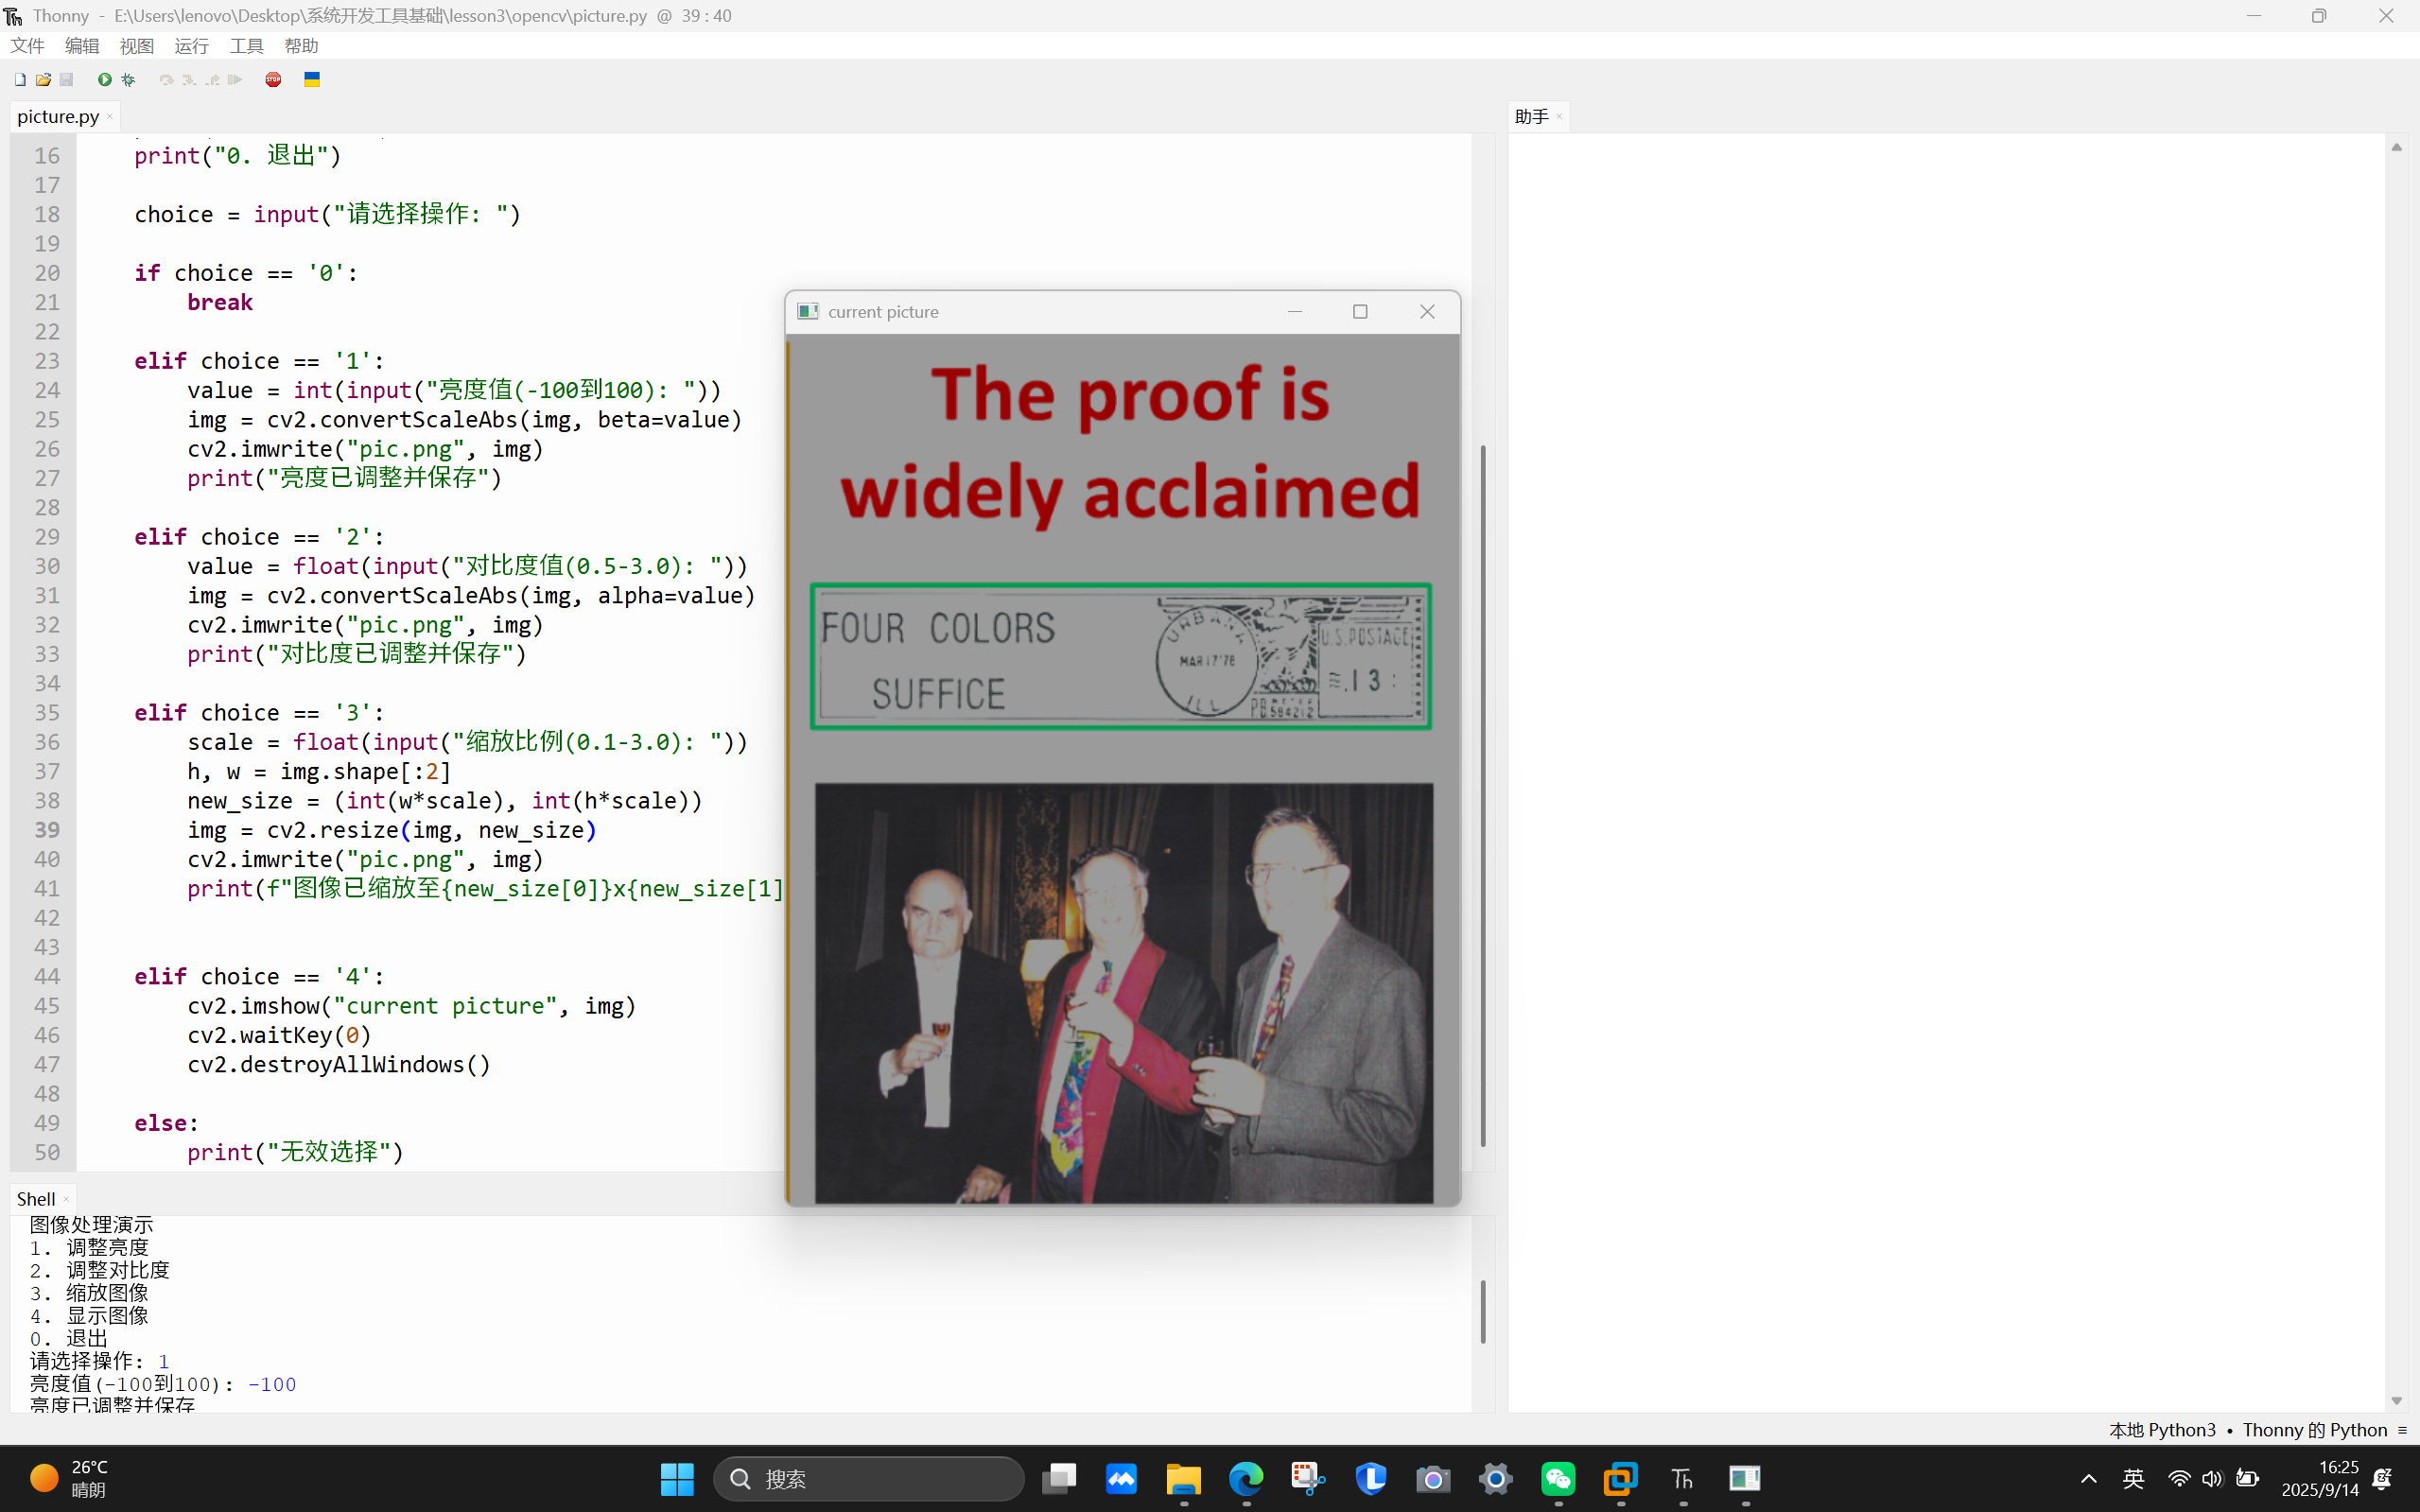
\includegraphics[width=0.8\textwidth]{lec3 (7).png}}
    \caption{lec3-7}
    \label{fig:lec3-7}
\end{figure}

\begin{figure}[htbp]
    \centering
    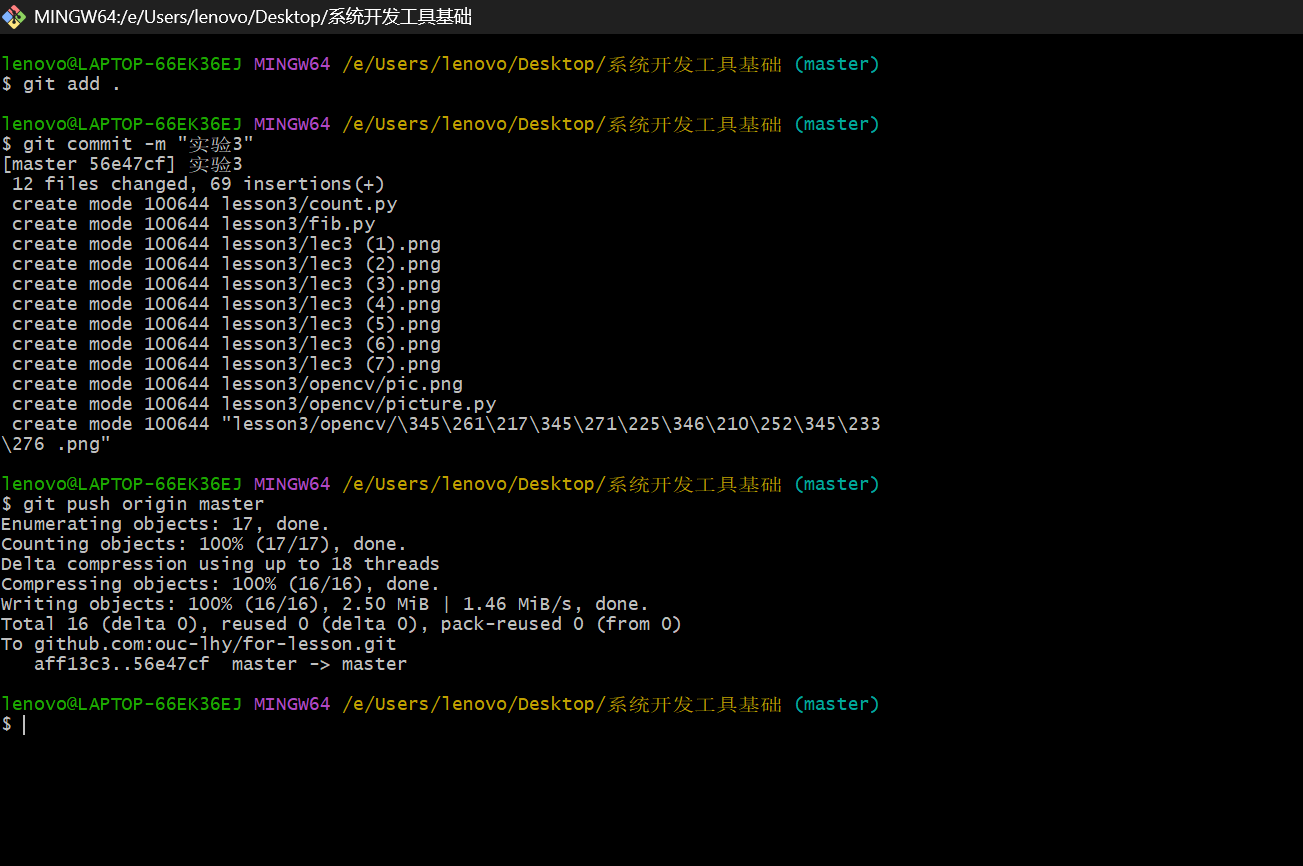
\includegraphics[width=0.8\textwidth]{commit.png}}
    \caption{commit截图}
    \label{fig:commit}
\end{figure}

\newpage

\section*{五、实验结果}
\begin{itemize}
    \item 成功实现对Python脚本的进程控制(前后台切换、暂停、终止);
    \item 能够使用 jobs、fg、bg、kill 等命令管理任务;
    \item 掌握Python基本语法与函数定义;
    \item 成功安装并使用OpenCV进行图像读取、转换与保存;
    \item 所有脚本均能正确运行,实验代码已整理并提交至https://github.com/ouc-lhy/for-lesson/tree/master/lesson3。
\end{itemize}

\section*{六、解题感悟}
本次实验深入学习了Linux任务控制机制,理解了进程状态转换与信号处理的重要性。通过count.py和fib.py的实际操作,掌握了如何管理长时间运行的任务。Python部分让我快速入门了这门强大的语言,其简洁语法和丰富库支持令人印象深刻。OpenCV的引入打开了计算机视觉的大门,图像处理的直观效果增强了学习兴趣。整个实验过程锻炼了我整合Shell、Python与系统工具的能力,为后续开发打下了坚实基础。

\section*{七、GitHub链接}
\url{https://github.com/ouc-lhy/for-lesson/tree/master/lesson3}

\end{document}